\chapter{Text Classification using deep learning}\label{chap:nnmethod}

\section{Introduction}

The problem of text classification or text categorization poses the following problem: assign a set of predefined categories to unstructured text that can be used to organize and structure the text appropriately according to the use case. Text classification is an pivotal problem with several applications in biomedicine. For instance, problems such as recognizing reportable cases of cancer from pathology reports, identifying certain phenotypes from clinical notes, performing word sense disambiguation (that is, given a context determine the semantic meaning for the usage of an ambiguous word), and associating medical subject headings (MeSH terms) to scientific articles, can all be reduced to instances of generic text classification problem. Further, text classification can be grouped into two categories namely, (i) multiclass classification (i.e. labels are mutually exclusive) and (ii) multilabel classification where each input can be assigned to more than one label. By definition, it is clear that multiclass classification is a special case of multilabel classification and hence the latter problem becomes more harder to solve than the former.


Traditionally, the problem of text classification is solved by leveraging conditional models such as support vector machines (SVMs) and logistic regression (LR), only to mention a few, trained on features extracted from the text including bag of words (BOWs)~\cite{sebastiani2005text}. Moreover, it has been observed in the literature that performance gains are achieved with better feature selection techniques, underlying dataset selection, and ensemble approaches~\cite{zhou2012ensemble}. On the other side, better performing models have also be devised by leveraging the field of feature engineering, where the objective is to derive domain specific features that are more relevant and important. For instance, emoticons, exclamations and hashtags form important features for sentiment analysis of Twitter feed~\cite{kiritchenko2014sentiment}. Moreover, especially in the field of biomedicine, exploiting interoperable concept explanations and inter-concept relations from domain specific knowledge base such as unified medical language system (ULMS)\footnote{https://www.nlm.nih.gov/research/umls/} have led performance gains in the accuracy of the underlying models~\cite{yepes2015knowledge}. To this end, models with linear classifiers with ensemble modeling and domain specific feature engineering has the capacity to attain competitive results for the task of text classification.


The advent of deep neural networks (deep nets) in the last decade or so has led to foundation for generic alternatives to supervised learning, especially for the task of object classification. Deep nets eliminate the laborious process of feature engineering and automatically learn high level representations of input which suites best for the underlying classification problem. Although, the resurgence of deep nets was initially meant for the field of computer vision, recently it has also been applied to natural language processing tasks (NLP)\cite{bengio2003neural, collobert2008unified, mikolov2013distributed} especially through learning distributed representations of words as vectors in high dimensional space. These vectors help the model in guiding elementary tasks such as part-of-speech (POS) tagging and parsing as well as abstract tasks such as text classification and machine translation. Typically, the novel deep learning approaches for text classification rely on architectures based on convolutional neural networks (CNNs) or recurrent neural networks (RNNs)~\cite{young2018recent}. In Figure \ref{fig:dlarch}, you can see a typical deep learning based text classification architecture pipeline.


% . For instance, scientific articles can be filtered by keywords, support tickets can be organized by urgency, tweets on twitter can be organized by sentiments, and so on. Due to the advent of deep learning in the last decade and especially their potential to attain high accuracies has benefited the task of text classification unconditionally. 



\begin{figure}[!htb]
    \centering
    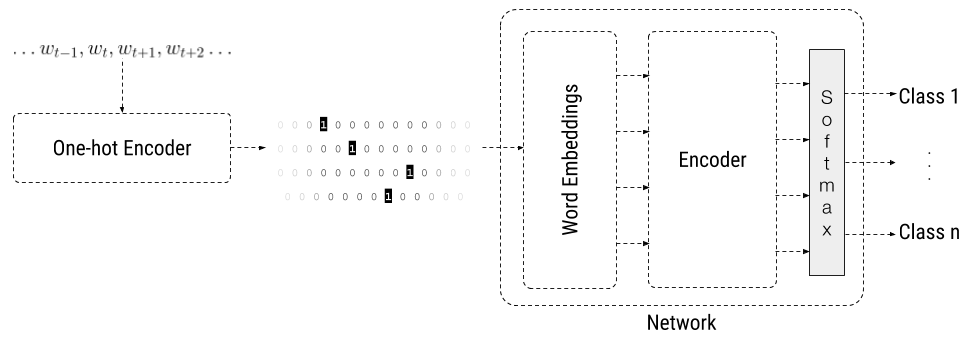
\includegraphics[scale=0.4]{Figures/text-classification-diagram.png}
    \caption{Typical neural network based deep learning architecture for multiclass classification of texts.}
    \label{fig:dlarch}
\end{figure}


Now we unfold each and every component of the architecture in Figure \ref{fig:dlarch}. 

\subsection{Unfolding the architecture}\label{section:architecture}

For an average human, understanding the inherent meaning of the words based on the context they are used is an easy task. In the same spirit, a deep learning model needs a clever pedigree so that it can understand the semantic similarity of related words and also differentiate each word from others. 


\paragraph{One-hot Encoding} As a natural convention, treating words as discrete atomic symbols, for instance, representing a \emph{cat} by \emph{Id100} and \emph{dog} by \emph{Id150} does not provide any meaningful information to the model regarding the relationship that may exist between the two symbols as they are some arbitrary encodings. This amounts to the model leveraging very little of what it has learned about \emph{cats} when it is processing data about \emph{dogs} (such that they are both animals, four-legged, pets, only to mention a few). Therefore, assigning unique, discrete IDs to the word tokens, that is, represented by a \emph{one-hot encoding vector} helps in understanding the model to differentiate between two different words. This in turn has an advantage as neural networks expect vectors as input. Although, this still does not provide any useful information to the model about the relationship between the words and in fact additionally, leads to sparsity. This entails that we may need more data in order to obtain meaningful statistical results. 


\paragraph{Word Embeddings} To overcome the problems of one-hot encoding,~\cite{bengio2003neural} developed the concept of word embeddings back in 2003. Despite being introduced before, word embeddings are still relevant today and highly active research domain in deep learning. The concept relies on the \emph{Distributional Hypothesis} of J.R. Firth (1957) that states that \emph{``You shall know a word by the company it keeps"}, that is, words that appear in the same contexts share semantic meaning. As we are in the context of neural networks, we are only concerned with predictive methods (i.e. neural probabilistic language models). Predictive models directly try to predict a word from its neighbors in terms of learned small, dense embedding vectors (considered parameters of the model).



A word embedding $\mathcal{W} : \text{words} \rightarrow \mathbb{R}^n$ is a parameterized function that maps words to high dimensional vectors (typically between 200 to 500 dimensions). In other words, it is a dense vector space that forces a fixed dimension on the vector space and forces similar words to appear nearby each other across some dimensions. Typically, the function $\mathcal{W}$ is a look-up table, parameterized by a matrix $\theta$ where each row corresponds to an embedding for a particular word: $\mathcal{W}_{\theta} (w_n) = \theta_n$ (refer Figure \ref{fig:word-embedding-matrix}). $\mathcal{W}$ is initialized randomly by having random row vectors for each word and the model learns to capture meaningful syntactic and semantic regularities in order to perform some task. Word2vec~\cite{mikolov2013distributed} and GloVe~\cite{pennington2014glove} are the two most popular word embedding models to obtain off-the-shelf trainable word embedding matrices. Moreover, word embeddings exhibit an interesting property, namely, it encodes semantic components as linear vector differences (refer Figure \ref{fig:linear-vector}).
 

\begin{figure}[!htb]
    \centering
    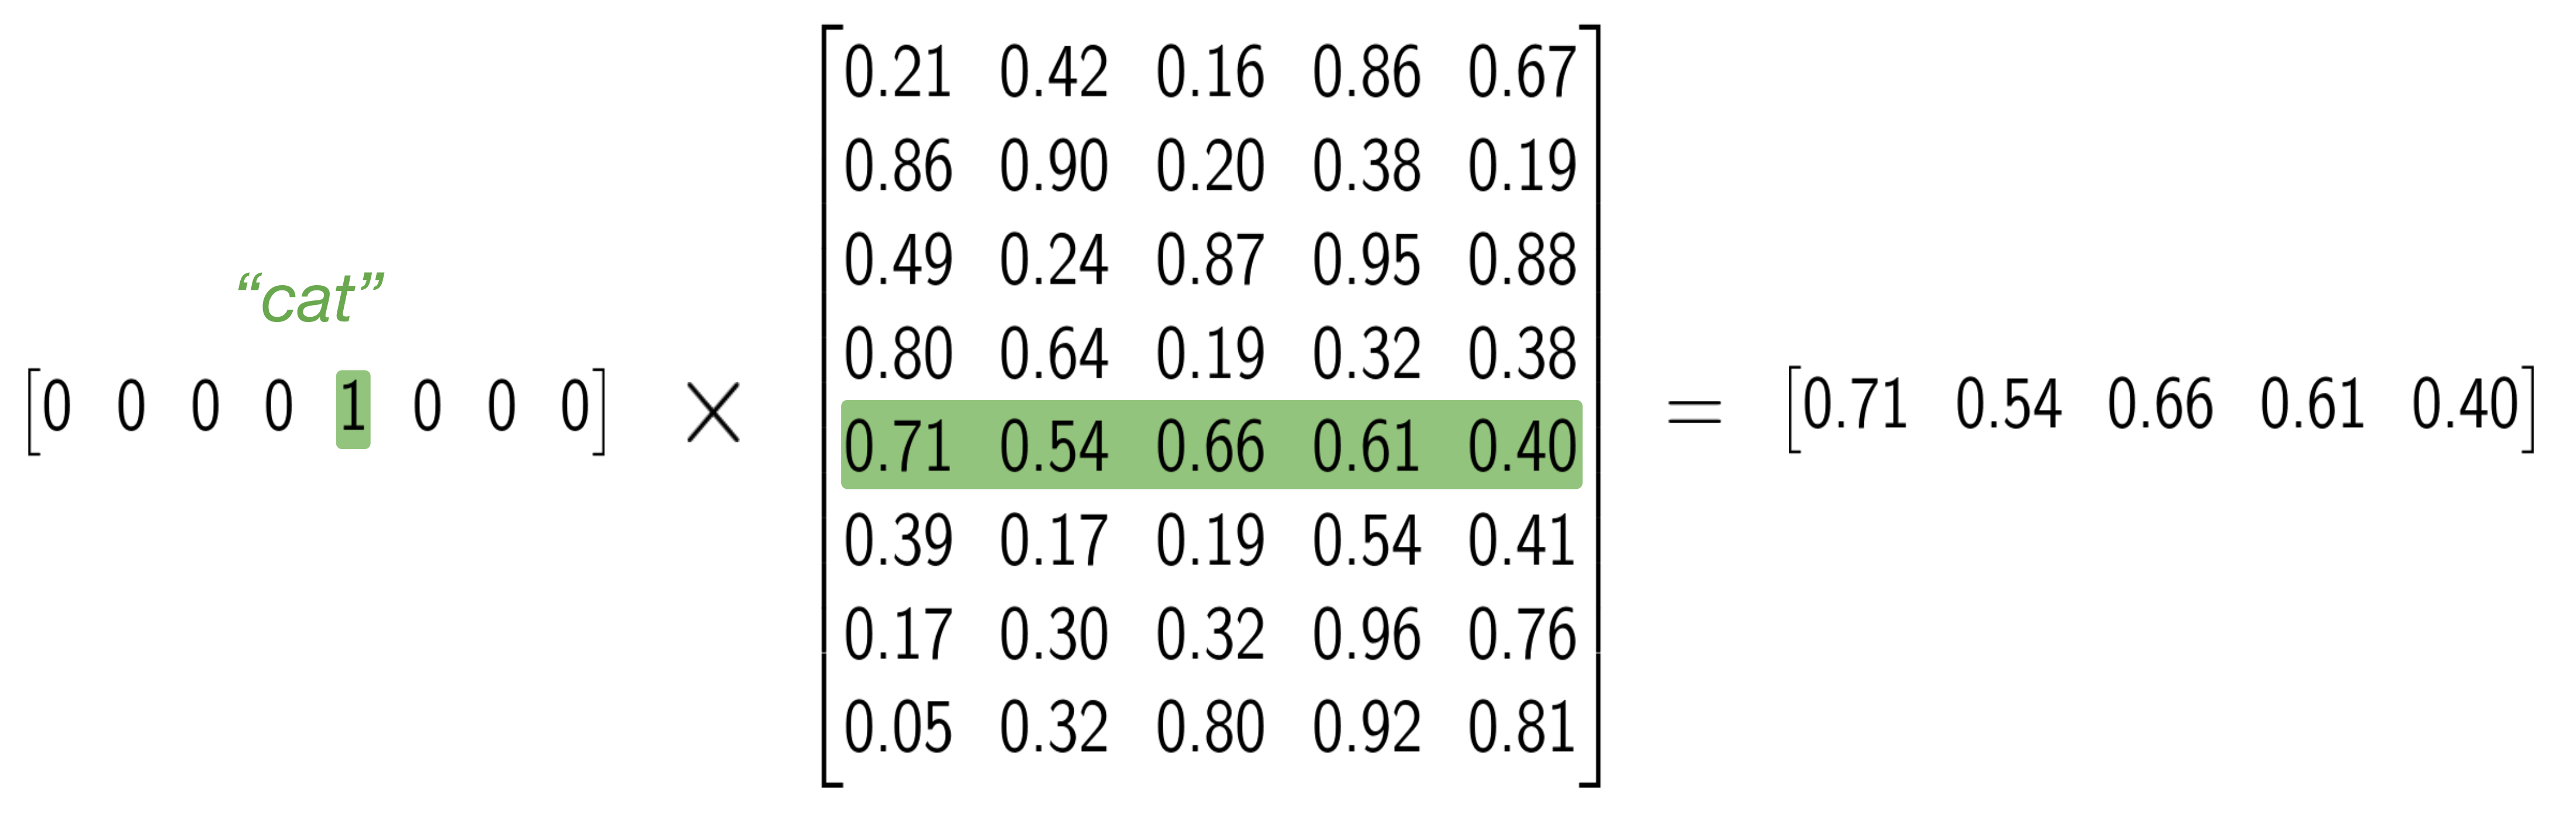
\includegraphics[scale=0.5]{Figures/word-embedding-matrix.png}
    \caption{The figure illustrates how to obtain embedding of a particular word \emph{"cat``} from a word embedding matrix. The one-hot encoding vector of the word \emph{"cat``} is multiplied to the word embedding matrix to obtain the embedding vector for \emph{cat}.}
    \label{fig:word-embedding-matrix}
\end{figure}


\begin{figure}[!htb]
    \centering
    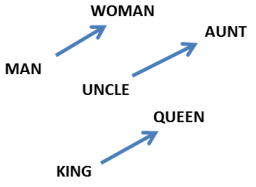
\includegraphics[scale=0.5]{Figures/Mikolov-GenderVecs.png}
    \caption{The difference between male-female vector is constant. That is, $\mathcal{W}(``\text{woman}") - \mathcal{W}(``\text{man}") \simeq \mathcal{W}(``\text{aunt}") - \mathcal{W}(``\text{uncle}") \simeq \mathcal{W}(``\text{queen}") - \mathcal{W}(``\text{king}")$ (Image Source~\cite{mikolov2013distributed}).}
    \label{fig:linear-vector}
\end{figure}


\paragraph{Encoder} Once we have the word embedding matrices from the raw text, in order to perform classification tasks, commonly used encoder architectures are convolutional neural networks (CNN) and recurrent neural networks (RNN). Next, we briefly summarize how is the classification task performed using the aforementioned architectures.

\paragraph{Neural Networks}
The neural network (NN) approach is widely used in the machine learning and deep learning algorithms to solve problems with complex, sparse data~\cite{lecun2015deep}. The word `neural' is used because they are loosely inspired by neuroscience. 
Neural networks are referred to deep feedforward networks pr feedforward neural networks. The goal of such a network is to estimate a function $f^*$.  In a traditional classifier $ y = f^*(\textbf{x})$, it maps the input $\textbf{x}$ to output category $y$. Whereas in the feedforward neural network the model defines a mapping $ y = f(x;\theta)$. It then learns the entities of parameter in $\theta$ which is in-turn best approximation of the function. 

One limitation of the linear classification like linear regression or logistic regression is that it is not able to detect any correlation between two input variables. NNs are used to perform non-linear classification tasks, 
%For example gradient descent which is a derivative of a linear function gives a smooth function, as nonlinear functions are a generalization of linear functions, 
see clearly in Figure~\ref{fig:linearclassification} and~\ref{fig:nonlinearclassification}. The neural network which uses a sigmoid function as their activation to perform computations $\sigma(x) = \frac{1}{1+e^{-x}}$, similarly a parameterized sigmoid function is: $\sigma_{w,b}(x) = \frac{1}{1+e^{-wx+b}}$ is shown in Figure~\ref{fig:neuron}. The inputs are given in the form of vectors (refer Figure~\ref{fig:vectorinputs}), if the network contains more than one layers, the composite functions are used to calculate the outputs. Other functions than sigmoid as activation like hyperbolic tangent  ($tanh$), Rectified Linear Unit($ReLU$) etc. 
\begin{figure}[!htb]
    \centering
    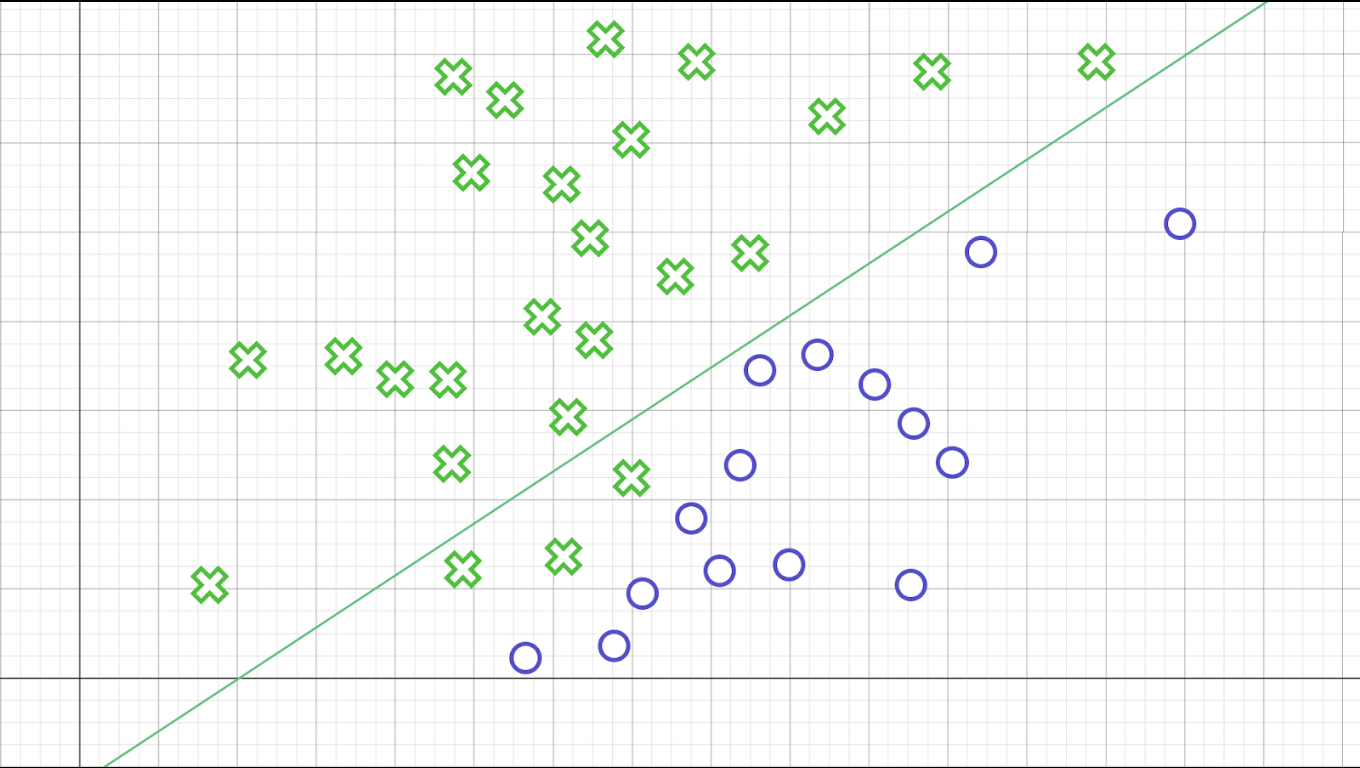
\includegraphics[scale=0.2]{Figures/non-linear_classification.png}
    \caption{A Linear Classification}
    \label{fig:linearclassification}
\end{figure}
\begin{figure}[!htb]
    \centering
    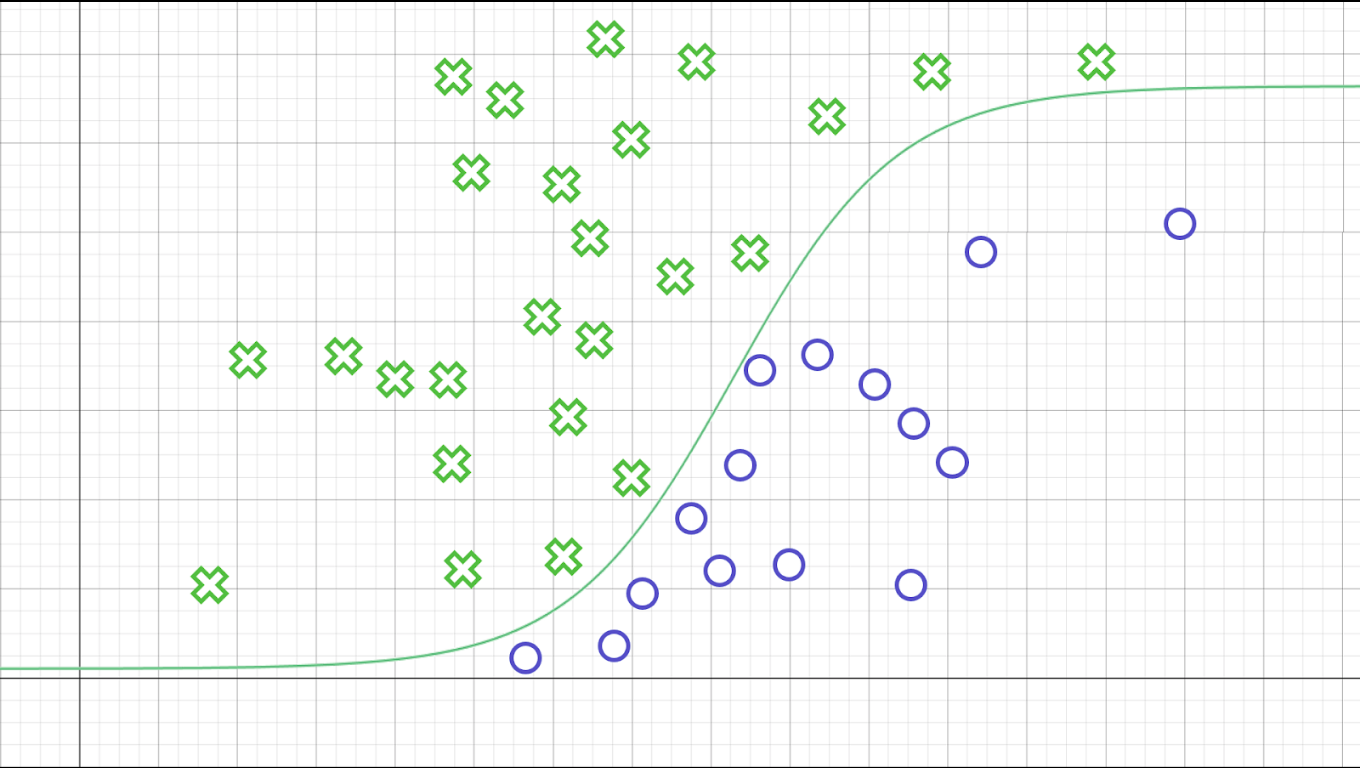
\includegraphics[scale=0.2]{Figures/linear_classification.png}
    \caption{A Non-linear Classification}
    \label{fig:nonlinearclassification}
\end{figure}
\begin{figure}[!htb]
    \centering
    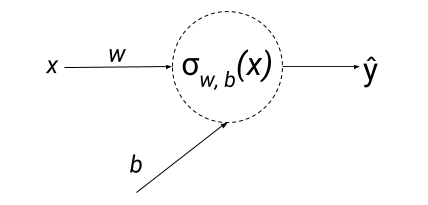
\includegraphics[scale=0.6]{Figures/neuron.png}
    \caption{Neuron}
    \label{fig:neuron}
\end{figure}
\begin{figure}[!htb]
    \centering
    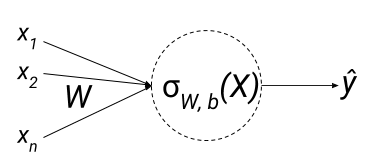
\includegraphics[scale=0.6]{Figures/Vector-Inputs-to-Neuron.png}
    \caption{Vector inputs in the neuron}
    \label{fig:vectorinputs}
\end{figure}

While training the neural networks we need to see how every parameter effects on the performance. For this purpose we calculate the model performance using loss function also known as \emph{loss function}. A loss function is the difference between the model output ($\hat{Y}$) and the given label (Y) for a data point for example using mean square error. 
\begin{equation}
    L(\hat{Y},Y) = \frac{1}{2n}\sum_{i=1}^{n}(\hat{y}-y)^2
\end{equation}
Given enough hidden units (neurons), a two layered neural network that can approximately imitate any continuous function, over a wide range of activation functions. Although the challenge is to find right values of the parameters given the input data. This is where backpropagation comes into practice. 
Backpropagation is done using gradient descent. The error gradient is calculated w.r.t. model parameters for each parameter. The parameters are changed in such a way that the parameters point in that direction where errors are increasing. 
\begin{equation}
    w_{n} = w_{n} - \eta\frac{dL}{dw_{n}}
\end{equation}

In a neural network architecture there are layers which are classified into three type which are mentioned below, all these layers contain nodes which are interconnected to each other in a dense manner also shown in Figure~\ref{fig:nn}:
\begin{itemize}
    \item \textbf{input layer} - this brings in the data into the architecture which is then pass on to the next layer for processing
    \item \textbf{hidden layer(s)} - after the input layers there are a certain number of interconnected layers these can be specified accordingly. Here, the network takes a bunch of weighted set and use an activation function to emit the output.
    \item \textbf{output layer} - last layer of nodes where we get the output.
\end{itemize}
\begin{figure}[!htb]
    \centering
    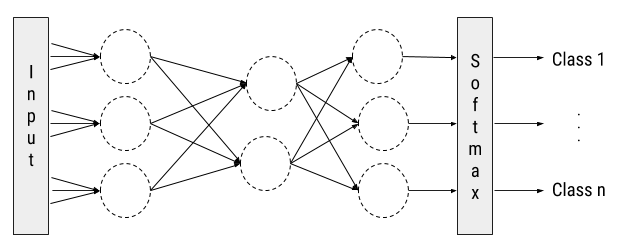
\includegraphics[scale=0.6]{Figures/neural-network.png}
    \caption{A simple neural network architecture}
    \label{fig:nn}
\end{figure}

%\paragraph{Convolutional Neural Networks} 

%\paragraph{Recurrent Neural Networks} 


\section{Model Specification}
Now, we describe the types of neural networks and discuss the model specification in context of this project using NCBI disease corpus and focusing on NLP. 
\subsection{CNN}\label{sec:cnn}
They are widely used in the context of images~\cite{krizhevsky2012imagenet}. Although, the architecture can be used if sentences or paragraphs or documents can be represented as matrices or vectors, as it is the case in images. Word embedding matrices typically act as pixel matrices of images in the context of text classification. One of the reasons as to why CNNs are successful is because of its inherent property of keeping a number of copies of the same type of neurons. This helps the model to have numerous neurons, while being able to process large complex models keeping same number of parameters. While writing programs in computer science we tend to write a function and keep calling it later on, the CNNs do a similar thing with the help of these large number of neurons. This in turn makes learning easier and reduces error. CNN has been successfully applied in NLP tasks~\cite{dos2014deep, zeng2014relation}. 

From the network point of view, CNN's are essentially several layers of convolutions (refer Figure~\ref{fig:CNN_layer} stacked upon each other with non-linear activation functions applied to the output of neurons in the same layer. 
\begin{figure}[!htb]
    \centering
    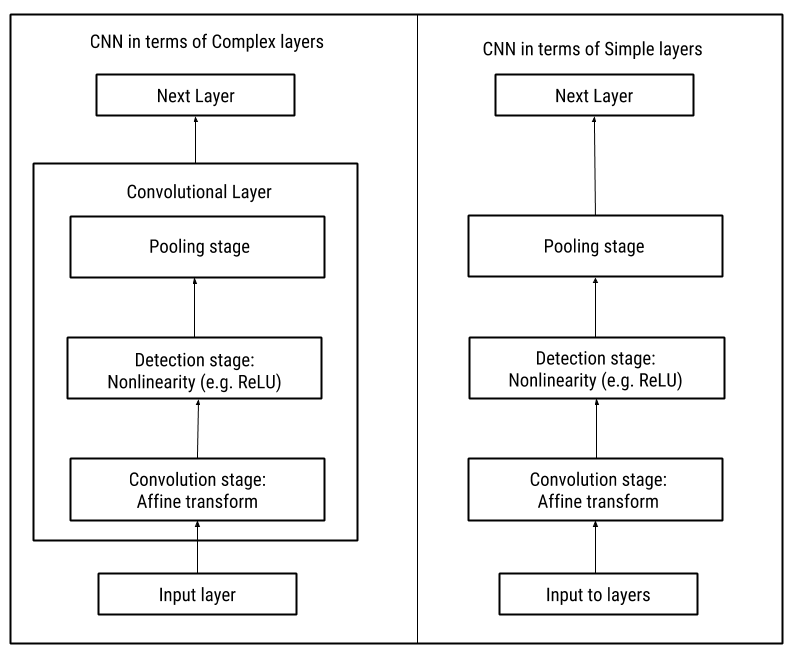
\includegraphics[scale=0.5]{Figures/cnn.png}
    \caption{A CNN Layer, from~\cite{Goodfellow-et-al-2016}}
    \label{fig:CNN_layer}
\end{figure}
A typical layer in a CNN has three stages: (i) convolution operation (refer Figure~\ref{fig:convolution}), (ii) a non-linear activation like rectified linear unit and (iii) a pooling function which lists the set of output with certain statistical explanation of outputs of neighbourhood. These three stages accommodate in the standard feed-forward architecture of linear and non-linear activations. As we can see from Figure~\ref{fig:CNN_layer},
the first stage is linear and the second layer when combined with the third stage form a non-linear activation. 
One of the most used pooling statistics is \emph{max-pooling}, see Figure~\ref{fig:maxpool}. 



\begin{figure}[!htb]
    \centering
    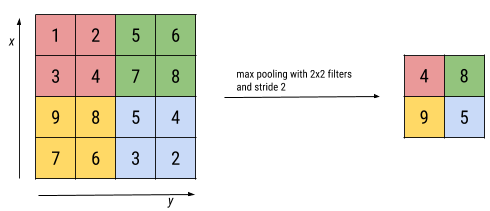
\includegraphics[scale=0.65]{Figures/max-pooling.png}
    \caption{Max-pooling, Source: \url{http://cs231n.github.io/assets/cnn/maxpool.jpeg}}
    \label{fig:maxpool}
\end{figure}
Figure~\ref{fig:convolution} illustrates that convolution is a binary operation that involves two operands namely, some text and a predefined kernel or filter, both of which are represented as matrices containing real numbers.
\begin{figure}[!htb]
    \centering
    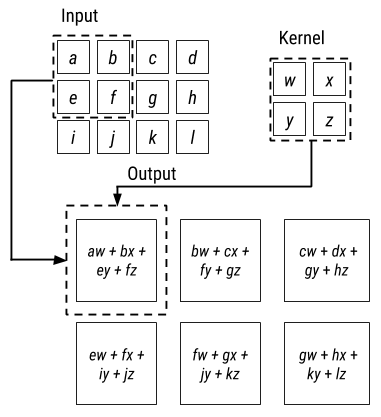
\includegraphics[scale=0.5]{Figures/convolution.png}
    \caption{Convolution}
    \label{fig:convolution}
\end{figure}
Typically, the matrix representation of text comprises of the word vectors of tokens that constitute it, that is, the word embedding matrix. The objective of the kernel is to operate on all contiguous segments of the text using a sliding window and produce number of contiguous segments (in text) many real numbers as output. This sequence of real numbers is called a feature map and is associated with a particular kernel being used to compute it. Generally, different kernels produce different feature maps that can be used as features for the task of text classification. The feature maps are then fed into a non-linear activation function as input, typically, softmax in our use case that outputs class or label probability estimates. The main idea here is to learn the matrix representations of kernels that in turn provide better feature maps, which optimizes the objective function efficiently. The learning takes place by predicting labels for training data and make adequate modifications to the kernel matrix through the back propagation algorithm that minimizes the loss function, that is, minimizes the conditional log-likelihood of training data. In the aforementioned abstract elucidation, we have omitted the technical details pertaining to CNNs like mathematical definition of convolution, the objective function and regularization. For the sake of completeness, we discuss these points in detail in the next section.

\subsection{CNN Model Description}
The architecture of the a CNN model with two layers including one convolution layer and a densely connected output layer is depicted in Figure~\ref{fig:Cnn_one_layer}.
\begin{figure}[!htb]
    \centering
    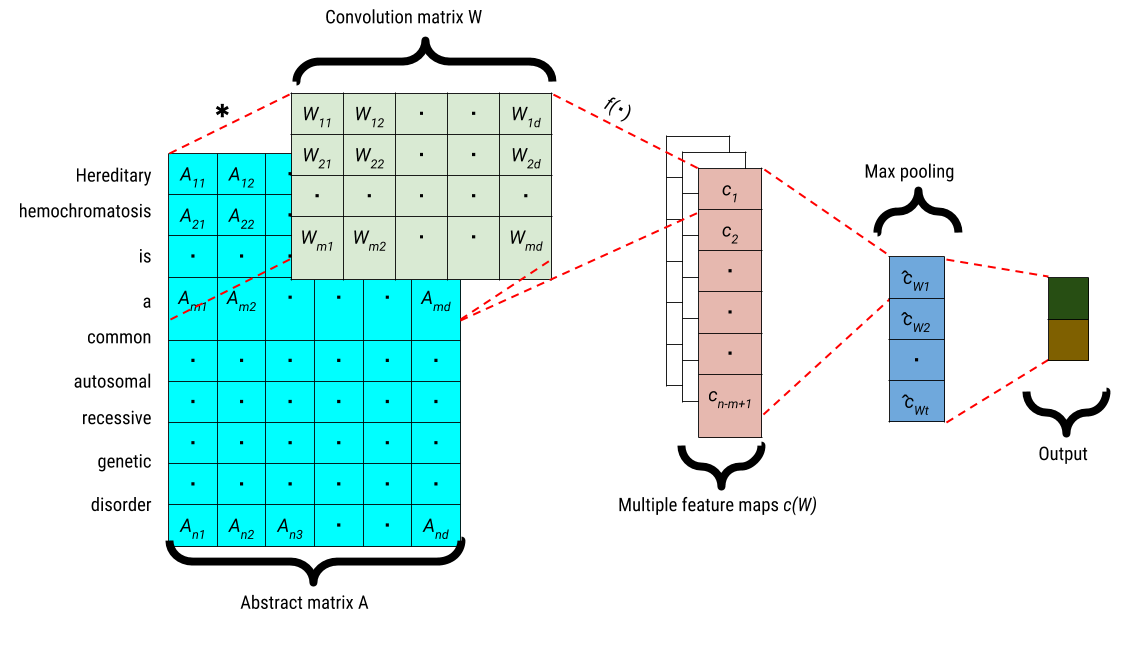
\includegraphics[scale=0.45]{Figures/cnn-model-example.png}
    \caption{Convolutional Neural Network with one convolution layer}
    \label{fig:Cnn_one_layer}
\end{figure}
The basic component of the model is the word vector $\mathbf{x} \in \mathbb{R}^d$, where $d$ is the dimension of the word vectors. An abstract is represented as a matrix $A \in \mathbb{R}^{n \times d}$, where $n$ is the number of words in it. As mentioned earlier in the section~\ref{section:architecture}, each row corresponds to the word vector for the corresponding token or word. For the sake of brevity, we assume that the ground truth (label) for the abstract is $y \in \mathbb{R}^2$ such that $y_2 = 1$ and $y_1 = 0$ ($y_2 = 0$ and $y_1 = 1$) when we are training on a positive (negative) instance. This is precisely depicted in the Figure~\ref{fig:Cnn_one_layer} with two output nodes of the final layer for the two classes (positive or negative) for each binary classifier.

We define a kernel $\mathbf{W} \in \mathbb{R}^{m \times d}$, where $m$ is the length of the sliding window. The two-dimensional convolution operation $\mathbf{*}$ can now be defined as follows,

\begin{center}
\[\mathbf{W} * A_{j:j+m-1} = \sum_{i=j}^{j+m-1} \sum_{k=0}^{d-1} \mathbf{W}_{i,k} A_{i,k}.
\]
\end{center}

Next, by using a non-linear function $f(\cdot)$, we map a window of length $m$ to a real number $c_j \in \mathbb{R}$ as 

\[c_j = f(\mathbf{W} * A_{i, j:j+m-1} + b),
\]
 
 where $b \in \mathbb{R}$ is the bias. In this thesis, $f(\cdot)$ is a Rectified Linear Unit (ReLU)~\cite{glorot2011deep, nair2010rectified}. We get the following feature map after convolving over the whole abstract,

 \[\mathbf{c(W)} = [c_1, \ldots, c_{n-m+1}].\]

 Further, to overcome the problem of varying abstracts, we perform the statistical operation of max-pooling~\cite{zhou1988image} (see also Figure~\ref{fig:maxpool})

 \[\widehat{c_{\mathbf{W}}} = \max_{i} \mathbf{c(W)}_i,\]

 that yields a feature $\widehat{c_{\mathbf{W}}}$ associated to the feature map generated by $\mathbf{W}$. Suppose that we want to learn $t$ many kernels $\mathbf{W}^1, \ldots, \mathbf{W}^t$, to obtain multiple features maps. This leads to $t$ many single max-pooled features which can be represented as follows,

 \[ \mathbf{\widehat{c_{\mathcal{W}}}} = [\mathbf{\widehat{c_{\mathbf{W}^1}}}, \ldots, \mathbf{\widehat{c_{\mathbf{W}^t}}}],
 \]

 where $\mathcal{W} = \{\mathbf{W}^1, \ldots, \mathbf{W}^t\}$. After this, finally we add a softmax layer. The parameters of the softmax layer $\mathbf{V} \in \mathbb{R}^2 \times t$ and $b^{V} \in \mathbb{R}^2$ with weighted inputs 

 \[y_j = \mathbf{V}_j \mathbf{\widehat{c_{\mathcal{W}}}} + b^{V}_j\]

and output label probability estimates as

\[P(y_j = 1 | A, \mathcal{W}, b, \mathbf{V}, b^{V}) = \frac{e^{y_j}}{\sum_i e^{y_i}},\]

where $\mathbf{V}_j$ $b^{V}_j$ are the $j^{th}$ row and $j^{th}$ element of $\mathbf{V}$ and $b^{V}$ respectively. $y_j$ is the $j^{th}$ label for the abstract corresponding to matrix $A$. 

If $\mathcal{A}$ is the set of training abstract matrices, then in order to learn each binary classifier, we minimize the following loss/objective function

\[- \sum_{A \in \mathcal{A}} \log(P(y_j^A = 1 | A, \mathcal{W}, b, \mathbf{V}, b^{V})),\]

where $j=1$ or $j=2$ depending upon the positive or negative training instance and $y^A$ is the ground truth label for the abstract represented by $A$. The parameters of CNN, that is $(\mathcal{W}, b, \mathbf{V}, b^{V})$ that minimize the loss function are modified by employing the back propagation algorithm with stochastic gradient descent approach. 

As a regularization term so that the model doesn't overfit, we use dropout~\cite{srivastava2014dropout}. More specifically, instead of feeding $y_j$ to the softmax function during training, we actually feed 

\[ \widehat{y}_j = \mathbf{V}_j( \mathbf{\widehat{c_{\mathcal{W}}}} \circ \mathbf{s}) + b^{V}_j
\],
 
where $\circ$ refers to hadamard product (element-wise multiplication) and $\mathbf{s} \in \{0,1\}^t$ is generated with each element $s_i$ drawn from the Bernoulli distribution with parameter $p$ set to $0.2$. In layman terms, this means that the gradients are backpropagated only through those neurons where $s_i = 1$. Note that, while testing the model, we scale the weights $\mathbf{V}$ such that 

\[y_j = p\mathbf{V}_j \mathbf{\widehat{c_{\mathcal{W}}}} + b^{V}_j.\]

This operation is essential because during training, only $80\%$ of the edges are active, that is obviously not true when we test the model. 


\subsection{RNN}
RNNs are widely used in natural language models because of the ambiguity of it. As a human being, every time when we try to solve something we don't reboot the brain, instead we remember things and try to build on from that. The traditional neural networks cannot have persistence, for example if we want to predict what word would come next in the sentence or when we want to do a prediction of the next term in the sequence. In such cases we need the information of what happened previously stored in the network, the RNNs are able to do such computations because they have loops in the network as can be seen in the Figure~\ref{fig:rnnarch}~\cite{chung2015recurrent}. Whereas when we deal with natural language there is context required for predicting what comes next, sometimes there is a difference between that there is a big difference between the relevant information and the point where it is needed. RNNs do not always perform best when handling ``long term dependencies''~\cite{bengio1994learning}. To overcome this problem, Long Short Term Memory networks (LSTMs) were introduced by~\cite{hochreiter1997long} that are a special kind RNNs which can handle learning the long term dependencies. 

\subsection{RNN Model Description}
Figure~\ref{fig:rnnarch} introduces the RNN architecture where the input $x_t$ is fed is a hidden layer at time step $t$. 
\begin{figure}
    \centering
    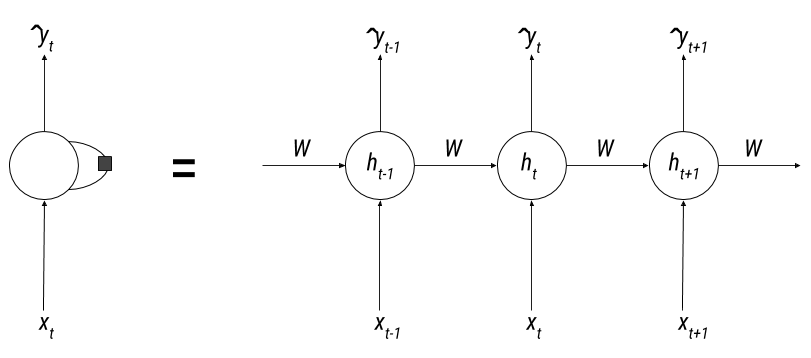
\includegraphics[scale=0.5]{Figures/rnn_figure_1.png}
    \caption{Recurrent Neural Network}
    \label{fig:rnnarch}
\end{figure}
The operations is modus-operandi to traditional neural networks as in: each layer consists of neurons, where each neuron performs a linear matrix operation on its corresponding input which is followed by a non-linear operation. At each time step, the output of the previous step along with the next word vector in the abstract are inputs to the hidden layer that yields $\widehat{y}$ as output and features $h_t$. The inputs and outputs to each neuron in RNN can be described as follows,

\begin{equation}
\begin{aligned}
	h_t = W f(h_{t-1}) + W^{(hx)}x_t
\end{aligned}
\end{equation}

\begin{equation}
\begin{aligned}
	\widehat{y} = W^{(S)}f(h_{t})
\end{aligned}
\end{equation}

Next, we mention the details associated with each parameter in the network:

\begin{itemize}
	\item Suppose the abstract is of $n$ words in total. Then $x_1, \ldots, x_n$ is the word vectors corresponding to the words of the abstract.

	\item $h_t = \sigma(W^{hh}h_{t-1} + W^{hx}x_t)$ corresponds to the hidden layer features at a particular time step $t$. Here $x_t \in \mathbb{R}^d$ is the input word vector at time step $t$. $W^{hx} \in \mathbb{R}^{D_h \times d}$ and $W^{hh} \in \mathbb{R}^{D_h \times D_h}$ are the weight matrices used to condition input word vector $x_t$ and output of previous time step $h_{t-1}$ respectively.

	\item $\widehat{y}_t = \text{softmax}(W^{(S)} h_t)$ corresponds to the output probability estimates over the vocabulary at each time step $t$. $W^{(S)} \in \mathbb{R}^{|V| \times D_h}$ and $\widehat{y} \in \mathbb{R}^{|V|}$ where $|V|$ is vocabulary.


\end{itemize}

The RNNs are trained using an application of back propagation algorithm known as back propagation through time (BPPT) algorithm. More specifically, it begins by unfolding the RNN in time: the unfolded network consists of $n$ inputs and outputs, but every copy of the network shares the same parameters. Then the back propagation algorithm is applied traditionally. The main disadvantage of RNNs is that they can not capture long-term dependencies due to vanishing/exploding gradients during backpropagation. More specifically, if the weights of the word embedding matrix which is input to the RNN are small, it can lead to a vanishing gradients where the gradient signal is so weak that the learning is slow or stops altogether. Conversely, if the weights are large, it can lead to very strong gradient signal that causes the learning to diverge, that is, exploding gradients.

To overcome the problem of long-term dependencies, LSTM was developed, that is, to gain more persistent memory. The mathematical formulation of the LSTM unit is described below,

\begin{equation}
\begin{aligned}
	i^{(t)} = \sigma(W^{(i)}x_t + U^{(i)}h_{t-1}) && \text{(Input \ Gate)} \\
	f^{(t)} = \sigma(W^{(f)}x_t + U^{(f)}h_{t-1}) && \text{(Forget \ Gate)} \\
	o_t = \sigma(W^{(o)}x_t + U^{(o)}h_{t-1}) && \text{(Output \ Gate)} \\
	\widetilde{c}^{(t)} = \text{tanh}(W^{(c)}x_t + U^{(c)}h_{t-1}) && \text{(New \ Memory \ cell)} \\
	c^{(t)} = f^{(t)} \circ \widetilde{c}^{(t-1)} + i^{(t)} \circ \widetilde{c}^{(t)} && \text{(Final \ memory \ cell)} \\
	h^{(t)} = o_t \circ \tanh(c^{(t)})
\end{aligned}
\end{equation}


%\todo{Draw Figure LSTM unit explaining gates}
\begin{figure}[!htb]
    \centering
    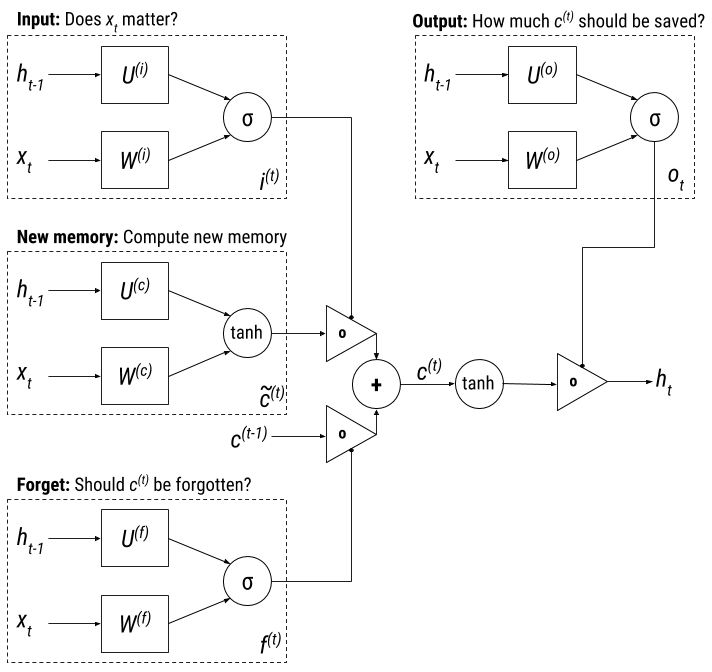
\includegraphics[scale=0.55]{Figures/lstm-unit.png}
    \caption{A LSTM unit}
    \label{fig:lstmunit}
\end{figure}

Finally, we explain the structure and the intuition behind LSTM units below:

\begin{itemize}
	\item \textbf{New memory generation: }It is the consolidation of a new input word vector $x_t$ with the past hidden state $h_{t-1}$. From the model point of view, this gate cooks the recipe of summarizing the new input in the light of contextual past.

	\item \textbf{Input Gate: }The new memory cell generates new memory blindly without even bothering whether the new input is important or not -- the objective of the input gate is to determine the importance to the new input by using it and the past hidden state. Hence, it is used to gate the new memory and produces $i^{(t)}$ which indicates information.

	\item \textbf{Forget Gate: }The forget gate is analogous to input gate in the sense that it makes an assessment on the usefulness of the past memory cell that is used for the computation of current memory cell. Thus, it looks at the input and the past hidden state and produces $f^{(t)}$.

	\item \textbf{Final memory generation: }Both the input gate and the forget gate act as an advisory to final memory cell, that is, whether to forget past memory or gate new memory respectively. The final memory cell then sums these results to produce final memory $c^{(t)}$.

	\item \textbf{Output Gate: } It's objective to the separate final memory $c^{(t)}$ from the hidden state. $c^{(t)}$ might not necessarily contain only relevant information all the time that is required to be saved by the hidden state. Moreover, as hidden states are used in every gate of an LSTM unit, the output gate makes an assessment regarding the importance of the information to be stored in the hidden state $h_t$. This produces $o_t$ and this is to gate the point-wise $tanh$ of the memory.
\end{itemize}

The bi-directional version of RNN or LSTM, at each time-step $t$, maintains two hidden layers, one for left-to-right propagation and another for right-to-left propagation. Clearly, this consumes twice as memory as RNNs. The final output $\widehat{y}_t$ is obtained by combining the scores computed by both the hidden states (refer to Figure~\ref{fig:lstmunit}).


